  \documentclass[twoside=true, %  doppelseitiger Druck
  DIV=15,% DIV Faktor für Satzspiegelberechnung, sie Doku zu KOMA Script
  BCOR=15mm, % Bindekorrektur
  chapterprefix=false,
  headinclude=true,
  footinclude=false,
  pagesize,%         write pagesize to DVI or PDF
  fontsize=11pt,%             use this font size
  paper=a4,%          use ISO A4
  bibliography=totoc,%         write bibliography-chapter to table of contents
  index=totoc,%         write index-chapter to table of contents
  cleardoublepage=plain,% \cleardoublepage generates pages with pagestyle empty
  headings=big,%       A4/B5
  listof=flat,%        improved list of tables
  numbers=noenddot
  ]{scrbook}

\usepackage[utf8]{inputenc}
\usepackage[slantedGreek,sc]{mathpazo}
\usepackage[scaled=.95]{helvet}
\usepackage{courier}
\usepackage[T1]{fontenc}
\usepackage{textcomp}
\usepackage{amsmath}
\usepackage{bm}
\usepackage{fixmath}
\usepackage{graphicx}
\usepackage[facing=yes]{floatrow}
\usepackage[labelfont=bf,sf,font=small,labelsep=space,format=plain]{caption}
\usepackage{subcaption}
\usepackage{scrpage2}
\usepackage{epstopdf}
\usepackage[ngerman]{babel}
\usepackage{ellipsis}
\usepackage{microtype}


%\usepackage{lmodern}
%\usepackage{amssymb,amsmath}
%\usepackage{ifxetex,ifluatex}

%\IfFileExists{upquote.sty}{\usepackage{upquote}}{}
% use microtype if available
%\usepackage{color}
\usepackage{fancyvrb}
\newcommand{\VerbBar}{|}
\newcommand{\VERB}{\Verb[commandchars=\\\{\}]}
\DefineVerbatimEnvironment{Highlighting}{Verbatim}{commandchars=\\\{\}}
% Add ',fontsize=\small' for more characters per line
\newenvironment{Shaded}{}{}
\newcommand{\KeywordTok}[1]{\textcolor[rgb]{0.00,0.44,0.13}{\textbf{{#1}}}}
\newcommand{\DataTypeTok}[1]{\textcolor[rgb]{0.56,0.13,0.00}{{#1}}}
\newcommand{\DecValTok}[1]{\textcolor[rgb]{0.25,0.63,0.44}{{#1}}}
\newcommand{\BaseNTok}[1]{\textcolor[rgb]{0.25,0.63,0.44}{{#1}}}
\newcommand{\FloatTok}[1]{\textcolor[rgb]{0.25,0.63,0.44}{{#1}}}
\newcommand{\CharTok}[1]{\textcolor[rgb]{0.25,0.44,0.63}{{#1}}}
\newcommand{\StringTok}[1]{\textcolor[rgb]{0.25,0.44,0.63}{{#1}}}
\newcommand{\CommentTok}[1]{\textcolor[rgb]{0.38,0.63,0.69}{\textit{{#1}}}}
\newcommand{\OtherTok}[1]{\textcolor[rgb]{0.00,0.44,0.13}{{#1}}}
\newcommand{\AlertTok}[1]{\textcolor[rgb]{1.00,0.00,0.00}{\textbf{{#1}}}}
\newcommand{\FunctionTok}[1]{\textcolor[rgb]{0.02,0.16,0.49}{{#1}}}
\newcommand{\RegionMarkerTok}[1]{{#1}}
\newcommand{\ErrorTok}[1]{\textcolor[rgb]{1.00,0.00,0.00}{\textbf{{#1}}}}
\newcommand{\NormalTok}[1]{{#1}}









\author{Michael Häuslmann, Markus Rodler, Marinus Noichl, Fabian Gerbig}
\title{Fair Projects - Analyse des MEAN Stacks}

\linespread{1.5}

\begin{document}

\maketitle
\newpage
\tableofcontents

\chapter{Einführung}
\label{einfuerung-michi}

Im Bereich der Webentwicklung wurde zur Entwicklung der Backends in den
letzten zehn Jahren u.a. die Programmiersprachen Java, C, PHP, Ruby und
Python verwendet. Auf Grund der Unterstützung der meisten Browser war
(von Applets und anderen für bestimmte Browser entwickelte Technologien)
JavaScript nur im Frontend im Einsatz. 2009 wurde eine JavaScript
Runtime (NodeJS) veröffentlicht. Diese ermöglicht die Ausführung von
JavaScript Code außerhalb des Browsers. Seitdem kann JavaScript sowohl
im Front- als auch im Backend verwendet werden.

Ziel dieser Arbeit ist es anhand einer Fallstudie die Vor- und Nachteile
einer mit dem MEAN Stack entwickelten Anwendung zu zeigen.

Die Fallstudie verwendet dabei den sog. MEAN Stack (\textbf{M}ongoDB,
\textbf{E}xpress, \textbf{A}ngular, \textbf{N}odeJS), bei dem sämtliche
Technologien mit JavaScript verbunden sind.
\section{Motivation}
\label{motivation}

\begin{figure}[h]
	\centering
	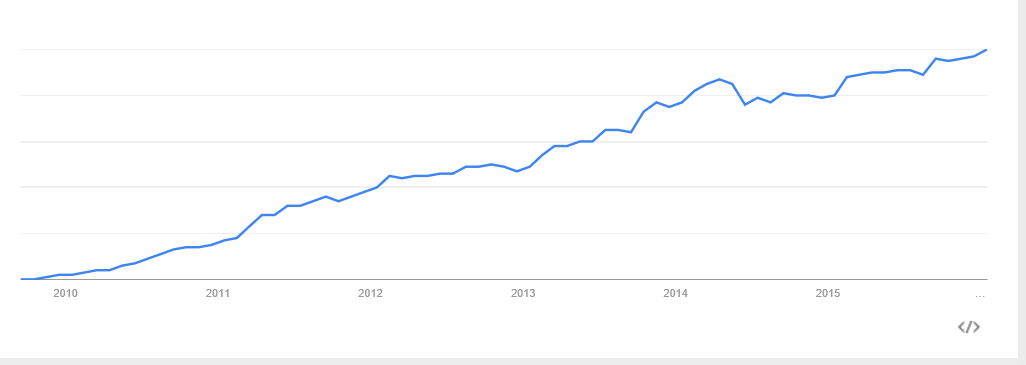
\includegraphics[width=0.7\linewidth]{figures/NodeJS.png}
	\caption{Steigerung der Suchanfragen für NodeJS. Datenquelle: Google Trends \cite{googleTrends:nodeJS}}
	\label{f:motivation:nodejs}
\end{figure}

Ein Großteil aller Webanwendungen ist in der Skriptsprache PHP geschrieben. 
So werden über 81\% aller Anwendungen damit geschrieben und ein demgegenüber verschwindend geringer Anteil von nur 0,1\% in JavaScript \cite{w3techs:serversidePLUsage}.
Dennoch stellt ein Grund sich näher mit dem MEAN Stack zu befassen die Tatsache dar, dass ein klarer Trend zu JavaScript erkennbar ist.
So ist das Interesse in den letzten Jahren enorm gestiegen wie auch in Abbildung \ref{f:motivation:nodejs} erkennbar ist.
Dort ist die Steigerung an Suchanfragen zu dem Thema NodeJS angegeben.
Google Trends liefert zwar keine absoluten Zahlen der Suchanfragen, jedoch lässt sich erkennen, dass die Anfragen sich in den letzten 5 Jahren stetig steigern konnten. 
Auch ist der Bekanntheitsgrad der anderen drei Komponenten stark gestiegen.
Selbst große Firmen wie Uber\cite{buildwith:uber.com}, Red Bull\cite{redbull:job} oder Netflix\cite{infoq:netflix} setzen Teile davon ein.
Oftmals wird dies durch eine verkürzte Entwicklungszeit zur Erstellung von Webanwendungen und durch eine gesteigerte Performanz begründet.
Zudem hat es gewisse Vorteile für Unternehmen. So erleichtert es Beispielsweise die Einführung von agilen Methoden in Unternehmen.
Meist werden Aufgaben in die Teile Frontend und Backend aufgeteilt und von unterschiedlichen Personen erarbeitet.
Frontendentwicklern, die sich typichscherweise sehr gut mit den Technologien HTML, CSS und JavaScript auskennen und Backendentwicklern, die nur mit den serverseitigen Komponenten wie beispielsweise PHP und MySQL arbeiten.
Da im MEAN Stack, NodeJS, Express und AngularJS auf JavaScript basieren und sogar MongoDB JavaScript ausführen kann, können nun die Aufgaben anderes aufgeteilt werden.
So ist es nicht mehr nötig nach Frondend und Backend zu trennen sondern die Aufgaben vertikal zu schneiden, wodurch jeder Entwickler alle Bereiche eines Features bearbeiten kann.
Vergleiche dazu das Elephant-Carpaccio von Alistair Cockburn \cite{cockburn:elephant}. 
Grund genug sich im Detail näher mit den einzelnen Komponenten zu beschäftigen.
\subsection{Einleitung, Idee, Motivation, bla
(Markus)}\label{einleitung-idee-motivation-bla-markus}

\begin{itemize}
\item
  Mockups
\item
  Architektur
\item
  REST API (bitte kurz definieren, damit ich mich darauf beziehen kann)
\item
  Erklärung der Funktionen
\item
  etc.
\end{itemize}

\chapter{MongoDB (Fabian)}\label{mongodb-fabian}

\section{Einleitung}\label{einleitung}

\begin{figure}[h]
	\centering
	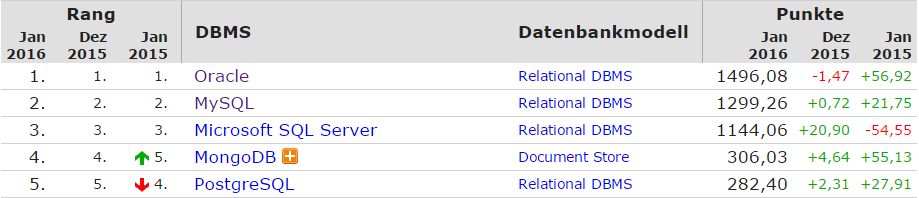
\includegraphics[width=0.7\linewidth]{figures/db-ranking.png}
	\caption{Datenbanken Ranking Datenquelle: db-engines \cite{db-engines:mongodb}}
	\label{f:mongodb:ranking}
\end{figure}

Die Entwicklung von MongoDB wurde im Jahr 2007 von dem Unternehmen 10gen
ins Leben gerufen. Als Programmiersprache wurde C++ verwendet.
Da die Datenmengen seit einigen Jahren durch Big Data immer rasanter steigen \cite{csc:bigdata}
werden die Skalierbarkeit und die Performanz bei großen Datenmengen zu
immer wichtigeren Themen. MongoDB wirbt mit Flexibilität, Skalierbarkeit und
Performanz. Dies soll durch denn Einsatz von verteilten Systemen
ermöglicht werden. Der Name mongo leitet sich aus dem Wort humongous ab,
welches gigantisch bedeutet. Hierdurch wird auf die Idee eine Datenbank
für große Datenmengen zu entwickeln angespielt.

Wie in der Abbildung \ref{f:mongodb:ranking} zu sehen steht MongoDB aktuell auf dem
vierten Platz der populärsten Datenbanken. Damit ist sie hinter drei
klassischen Relational Database Management System (RDBMS) die populärste
NoSQL-Datenbank. Bei der aktuellen Version handelt es sich um die 3.2.

\section{Konzepte}\label{konzepte}

\subsubsection{Grundlagen}
Eine herkömmliche RDBMS besteht aus Datenbanktabellen, die einem festen
Schema unterliegen. Bei MongoDB dagegen handelt es sich um eine
Schema-freie, dokumentenbasierte Open-Source-Datenbank. Diese beinhaltet
Sammlungen, die jeweils aus mehreren Dokumente ohne ein festes Schema
bestehen. Jedes Dokument darin kann sich von den Feldern und Strukturen
von den anderen unterscheiden. Dokumente bestehen aus mehreren
Schlüsselwert-Paaren und stellen die Basiseinheit für Daten dar.
Diese Daten werden im sogenannten BSON Format gespeichert und
ausgetauscht. Dabei handelt es sich um die binäre Variante von JSON.

\subsubsection{Datentypen}
Die hierbei verwendbaren Datentypen sind die bekannten Standard-Datentypen
Integer, Float, Boolean, String, Array. Zusätzlich gibt es noch die Date, Embedded-Doc, DBRef und
ObjectID.

\subsubsection{Referenzierung}
Es gibt unterschiedliche Wege in der Datenbank zu referenzieren.
Eine Möglichkeit ist die Referenzierung durch die Verschachtelung der Dokumente.
Hierbei referenziert ein Dokument auf ein anderes einzelnes Dokument.
Allerdings führt dies zu einer hohen Komplexität, wenn z.B. ein Update auf
eine verschachtelte Information durchgeführt werden soll.

Bei der ObjectID handelt es sich um die Standard ID, die jedes Dokument
aufweist. Diese wird bei der Erzeugung eines jeden Dokuments generiert
und ist durch ihren komplexen Aufbau eindeutig. Bei Verwendung der
ObjectID handelt es sich im Gegensatz zu verschachtelten Dokumenten um
einen ``echten'' Join. Hier referenzieren mehrere Dokumente auf ein Dokument
in der gleichen Collection.

Der DBRef entspricht dem Fremdschlüssel aus dem
RDBMS. Also dient er als Identifier für Dokument, Collection und
Datenbank. Dadurch können mehrere Dokumente auf ein Dokument in einer anderen
Collection referenzieren.

MongoDB verwendet eine integrierte Query Language. Durch
diese können Abfragen, Replikationen und Sharding auf den mongos ausgeführt werden.

\subsubsection{Replikation}
Die Replikationen spielen bei NoSQL-Datenbanken eine zentrale Rolle. Diese sorgen für die Synchronisierung von Daten über mehrere
Server. Im Gegensatz zu RDBMS sind bei NoSQL-Datenbanken Rundanzen erwünscht.
Denn diese dienen sowohl als Backup der Daten, als auch um die Performanz bei
Leseoperationen zu steigern. Nachteil hierbei ist, dass die Konsistenz nicht mehr gewährleistet werden kann.
Ein weiterer Nachteil ist das mehr Speicherplatz benötigt wird. Dies sollte jedoch, da es um
verteilte Systeme geht, kein Problem darstellen.

Bei MongoDB funktionieren die Replikationen nach dem Master-Slave-Prinzip. \cite{mongodb:replication}
D.h. es existieren in der Datenbank lauter Replikationssets. Diese bestehten
aus einer primären Replikationen und beliebig vielen sekundären Replikationen, also Kopien von den
primären Replikationen. Alle Schreiboperationen gehen nur an die primären Replikationen. Diese synchronisieren ihre sekundären
Replikationen erst nach und nach. Das bedeutet, dass die Daten für eine gewisse Zeit
inkonsistent sind. Es kann daher keine Konsistenz zum Transaktionszeitpunkt garantiert werden wie bei RDBMS.

Im schlimmsten Fall funktioniert eine Schreiboperation auf der ausführenden primären Replikation und
diese fällt aus bevor sie die Schreiboperation an die sekundären Replikationen
weitergegeben konnte. Dies führt nämlich zu Datenverlust, ohne das MongoDB
etwas davon mitbekommt. Die Datenbank denkt dann das die Operation
erfolgreich ausgeführt wurde, obwohl das gar nicht der Fall ist.

Jetzt könnte man sich fragen, warum eine Schreiboperation nur auf einer der primären Replikationen ausgeführt wird.
Dadurch wird ja ein Flaschenhals bei der Performanz von Schreiboperation erzeugt.
Das stimmt zwar, aber der Vorteil des automatischen failover überwiegt. Falls also
die primäre Replikation bei dem Versuch eine Schreiboperation auszuführen nicht erreicht werden kann,
wird eine der ehemals sekundären Replikationen zur neuen primären Replikation definiert. Da es sich bei den sekundären Replikationen
um eine Kopie der primären handelt ist dies ohne großen Aufwand möglich.

Für Leseoperationen kann man MongoDB nach seinen eigenen Wünschen konfigurieren. \cite{mongodb:replication}
Eine Möglichkeit ist die Last auch auf sekundäre Replikationen zu verteilen.
Vorteil hiervon wäre eine bessere Performanz bei Leseoperationen, da man quasi einen
Skalierungeseffekt erhält. Allerdings kann man nicht sicher
sein, dass alle sekundären Replikationen die aktuellsten Daten beinhalten.
D.h. man bekommt unter Umständen alte Datenstände zurück. Daher kann es durchaus sinnvoll sein
MongoDB so zu konfigurieren, dass auch Leseoperationen nur von der primären Replikation durchgeführt werden.

\subsubsection{Sharding}
Um den in der heutigen Zeit nicht ungewöhnlichen stark wachsenden Datenmengen
zu begegnen gibt es das automatische Sharding \cite{mongodb:sharding}. Dieses sorgt für die
Verteilung der Daten über mehrere Server. Dies wird auch als
horizontale Skalierung bezeichnet. Hierdurch ergeben sich vielfältige Vorteile. Zum
einen verursacht das vertikales Skalieren, also der Einsatz immer
besserer Hardware exponentielle Kosten und ist auch nicht unbegrenzt möglich. Zum anderen ist der lokale
Speicher möglicherweise einfach nicht groß genug. Da man durch das automatische Sharding einfach zusätzliche Server
in das Datenbank System integrieren kann hat man diese Probleme nicht.

Die Komponenten sind Shards, Config Server und mongos. Jedes Shard entspricht einem oben
beschriebenen Replikationsset. Die Config Server beinhalten die
Metadaten von dem Cluster. Sprich eine Map von den angefragten Daten und
ihren Speicherorten. Um eine ausreichende Redundanz und Verfügbarkeit gewährleisten zu können
muss es drei Config Server geben. Dann gibt es noch die mongos. Diese
werden von der Applikation angesprochen und führen die query Kommandos
aus.

Um Sharding durchführen zu können wird außerdem Map and Reduce eingesetzt. Map and Reduce entspricht dem Group Operator in RDBMS.
Hierbei werden auf allen Servern parallel Map Operationen ausgeführt. Danach fast die Reduce Operation alles zu einem Ergebnis zusammen.

\subsubsection{BASE}
Bedingt durch die oben genannten Konzepte ist eine strenge Einhaltung der ACID (atomar, consistency, isolation, durability) Kriterien nicht möglich. Es wird ein Tradeoff von Konsistenz und Isolation zu einer besseren Performanz und Skalierbarkeit eingegangen. Da man auf Konsistenz allerdings nicht vollständig verzichten kann wird das abgeschwächte BASE (Basically Available, Soft state, Eventual consistency) angestrebt. Hierbei wird nur eine "weiche" Konsistenz gewährleistet.

\section{Usecases}\label{usecases}

Ein großer Vorteil von MongoDB ist, dass es schnell einsetzbar / konfigurierbar ist.
Außerdem stellt eine sich öfter ändernde Datenstruktur kein Problem da.
Damit eignet sie sich hervorragend für rapid prototyping bei kleineren Projekten.

Allerdings eignet sie sich durch das Replizieren und ihre Skalierfähigkeit auch für große Datenmengen
und besonders für Leselastige Anwendungen.

Den Hauptnachteil stellt die nicht wirklich gegebene Konsistenz dar.
Dadurch steigt der Aufwand für die Anwendungsentwicklung, die daraus entstehende Probleme abfangen muss.

MongoDB wird damit für viele Anwendungsfälle nicht geeignet sein, da man einen Tradeoff eingehen muss.
Welche Datenbank verwendet werden sollte hängt somit immer von den konkreten Anforderungen ab.

\section{Mongoose}\label{mongoose}

Bei Mongoose handelt es sich um ein Modul für das NodeJS Framework.
Durch dieses Modul wird Object Data Modelling (ODM) im Zusammenhang mit MongoDB ermöglicht.

Der Hauptvorteil von Mongoose besteht in der Abstraktion von Daten der MongoDB.
Man kann sich Mongoose als abstrakte Schicht über MongoDB, der die schemalosen Daten auf Objekte mappt vorstellen.
Viele Entwickler, die es vorher mit SQL-Datenbanken zu tun hatten dürften damit wesentlich besser zurecht kommen,
als mit den dynamischen Sammlungen von MongoDB.

\begin{figure}[h]
	\centering
	\begin{lstlisting}
		var mongoose = require('mongoose');
		mongoose.connect('mongodb://localhost/test');

		var Cat = mongoose.model('Cat', { name: String });

		var kitty = new Cat({ name: 'Zildjian' });
		kitty.save(function (err) {
		if (err) // ...
		console.log('meow');
});
	\end{lstlisting}
	\caption[mongooseSchema]{Programmbeispiel \cite{mongoose:bsp}}
\end{figure}

Anhand dieses Beispiels erkennt man wie mithilfe von Schemas und Models Strukturen definiert werden.

Außerdem bietet diese Bibliothek auch noch einige andere Funktionalitäten. Unter anderem zum Einsatz von Middleware, Plug-Ins und zur Validierung.

Mongoose verwendet das Konzept Active Records. Dies ist ein durchaus umstrittenes Konzept,
da es auf der einen Seite als leicht und schnell erlernbar gesehen wird,
allerdings auf der anderen Seite das Testen erschwert und zu Flaschenhälsen in der Performanz führt. \cite{ormPattern:activeRecord}

Die Dokumentation auf der offiziellen Webseite ist sehr unübersichtlich. Hierdurch wird das Arbeiten mit dieser Bibliothek erschwert.

Die aktuelle Version von Mongoose wurde im Januar 2016 als 4.3.5. veröffentlicht.

\chapter{Express (Michi)}\label{express-michi}

\textbf{Grobschrift, da muss noch viel geändert und zitiert werden.}

Express ist der de-facto Standard für Node.js Webframeworks. Es gibt
sehr viele Alternativen (koa\cite{koa}, hapi\cite{hapi}, total.js\cite{totaljs}), jedoch gibt es
kein anderes Framework, das so viele Benutzer und Mitwirker hat.

% hier Vergleich der verschiedenen Stars etc. machen und in den Anhang

Verglichen mit Webframeworks, die sich in anderen Sprachen etabliert
haben, ist Express leichtgewichtig und liefert wenig Funktionalität.
Frameworks aus Programmiersprachen wie z.B.

\begin{itemize}
\item
  Ruby on Rails in Ruby
\item
  Spring in Java
\item
  Symfony in PHP
\item
  Django in Python
\end{itemize}

liefern Funktionalität für typische Webanwendungen (Sessions, Cookies,
Authentifizierung, Form Handling, Templating, \ldots{}).

Strongloop\cite{strongloop}, die Firma hinter Express, bietet inzwischen Training für Node.js und API
Entwicklung an.

Erweiterte Funktionalität muss bei Express über 3rd-Party Erweiterungen
hinzugefügt werden. Die Wartung dieser Erweiterungen wird dabei nicht
kontrolliert oder von den Entwicklern von Express beeinflusst.

Die Probleme die sich hieraus enwickeln können, werden in den nächsten Kapiteln diskutiert.

\section{Installation und
Versionierung}\label{installation-und-versionierung}

Die Installation von Express erfolgt über npm (den Node Package Manager)
und macht wenig Probleme. Voraussetzung ist jedoch, dass die
installierte Version von Node, zu der gewünschten Express Version passt.

Im Umlauf befinden sich die Versionen 2, 3, 4 und 5, wobei 2 und 3 als
deprecated markiert wurden und sich 5 noch in aktiver Entwicklung
befindet. Problematisch hierbei ist wieder, dass sämtliche Erweiterungen
für Express zu den entsprechenden Versionen von Express passen müssen.

Entscheidet man sich für vordefinierte MEAN Stacks wie z.B. MEAN.IO oder
MEAN.JS, dann lassen sich einzelne Komponenten nur austauschen, falls
der Ersatz die entsprechenden Versionen von Express und Node
unterstützt. Auf Grund der häufig sehr hohen Anzahl an Erweiterungen ist
dies oft problematisch.

\section{Kernfunktionalität}\label{kernfunktionalituxe4t}

Die Kernfunktionalität von Express ist, wie bereits erwähnt wurde, sehr
beschränkt. Im Prinzip übernimmt Express lediglich das Routing\footnote{Mapping der URL auf die Funktionen einer Anwendung} der Requests auf, vom Entwickler definierte, Callbacks.

Einige Funktionen wie z.B. das Parsing einer Anfrage oder senden von Cookies
sind eigentlich Kern einer jeder Webanwendung. Express benötigt jedoch sogar für
diese Funktionen Erweiterungen.

Erweiterte Funktionalität wird über Middlewares ermöglicht. Middlewares
können das Request und Response Objekt verändern und weiter- bzw.
umleiten oder terminieren (z.B. falls keine Zugriffsrechte bestehen).

\section{Anwendung}\label{anwendung}

Javascript ist eine Prototyp-basierte Sprache, die zumindest vor dem
ES6 Standard kein Klassenkonzept kennt. Deshalb und auf Grund der Art wie Express
die Routes verarbeitet, ist es nicht möglich Controller als Klassen wie
in einer typischen MVC (Model View Controller) Architektur umzusetzen\footnote{Dies gilt auch für Frameworks wie Total.js die damit werben ein komplettes MVC Framework zu sein]}.

Aus Gründen der Übersichtlichkeit und um die Funktionalität zu kapseln
und damit ggf. wiederverwendbar zu machen, haben wir die Callbacks der Routes in
eine Controller-ähnliche Struktur gebracht. Die jeweiligen Funktionen
auf den Controllern entsprechen dabei statischen Funktionen anderer
Programmiersprachen\footnote{wie bereits erwähnt ist es in Express nicht möglich
Methoden auf instanziierten Controllern aufzurufen}.

\begin{figure}[t]
	\centering
	\begin{lstlisting}
	/**
	* Creates a ProjectController
	* @returns {ProjectController}
	*/
	module.exports = function() {
	
		'use strict';
		
		/**
		* Updates an given project and returns the updated object.
		*
		* @param {http.IncomingMessage} req Express Request Objectistist
		* @param {http.OutgoingMessage} res Express Response Object
		* @callback next Callback which calls the next matching route.
		*/
		ProjectController.prototype.update = function(req, res, next) {
			// ...
		};
		
		return new ProjectController();
	};
	\end{lstlisting}
	\caption[controller]{TODO: Programmbeispiel für das Controller Prinzip}
	\label{f:controller}
\end{figure}

\section{Dependency Injection}\label{dependency-injection}

Da die Funktionalität in Express üblicherweise\cite{express-routing}
via Callbacks realisiert wird, ist es nicht möglich Abhängigkeiten
separat zu verwalten. Die Callbacks von Express kennen lediglich die
Parameter \texttt{req}, \texttt{res} und \texttt{next}. Express
unterstützt Dependency Injection nicht als Kernfunktionalität und bietet
auch sonst keine Möglichkeit zur Inversion of Control (TODO).

Dies hat zur Folge, dass die Erstellung von Objekten vielfach dupliziert
wird und außerdem schlecht testbar ist. Die Abhängigkeiten werden
typischerweise im Callback instanziiert und können somit nicht durch
Mockobjekte ausgetauscht werden.

Es existieren 3rd-Party Erweiterungen wie z.B. express-di\cite{express-di} oder
express-dinja\cite{express-dinja}, diese
waren aber entweder nicht mit unserer Version von Express kompatibel
oder konnten nicht mit unserem Controller-Konzept vereinbart werden.

Eine eigene minimale Implementierung \footnote{die von den genannten
Erweiterungen ähnlich implementiert wird} wurde via Middlewares
realisiert. Ein Dependency Injection Container wird dabei an das Request
Objekt \texttt{req} angehängt. Diese Lösung ist nicht optimal und
verletzt u.a. das Single Responsibility Principle
\cite{srp}. Express verhindert jedoch eine
andere Implementierungsweise.

\begin{figure}[t]
	\centering
	\begin{lstlisting}
		var dicMiddleware = function(req, res, next) {
		  req.dic = {
		    subjectRepository: require('../models/SubjectRepository'),
		  };
		  next();
		};
		subjectRouter.use('/', dicMiddleware);
	\end{lstlisting}
	\caption[dicMiddleware]{TODO: Programmbeispiel für eine dicMiddleware}
	\label{f:dicMiddleware}
\end{figure}

Mit dieser Implementierung war es uns möglich die Controller zu testen,
da lediglich Mockobjekte für \texttt{req} und \texttt{res} erzeugt
werden müssen.

\section{Typische Probleme der
Webentwicklung}\label{typische-probleme-der-webentwicklung}

Express unterstützt die häufigst verwendeten Javascript Template Engines
(Jade\cite{jade}, EJS\cite{ejs}, Haml\cite{haml}), liefert jedoch
keine eigene Implementierung.

Fair Projects nutzt Express als API Framework und somit finden Templates in der
aktuellen Implementierung keinerlei Verwendung. Ein technischer
Durchstich hat allerdings sowohl mit Jade als auch EJS einwandfrei funktioniert.

Authentifizierung und Authorisierung kommen in den meisten klassischen
und modernen Single-Page Anwendungen vor. Express unterstützt weder
Sessions (es gibt aber eine offizielle Erweiterung \cite{express-session}), noch
Cookies und damit auch keine Authentifizierung. Die de-facto Erweiterung
zur Authentifizierung ist Passport\cite{passport}.

Fair Projects sollte ursprünglich ein externes
Authentifizierungsverfahren von Github, Twitter oder Facebook verwenden.
Die Erweiterungen hierzu von Passport (Passport ist ähnlich wie Express
modular aufgebaut und unterstützt selbst fast keine Verfahren) waren
entweder veraltet und durch neuere ersetzt oder haben sich so
weiterentwickelt, dass die Dokumentation nicht mit der Implementierung
übereinstimmte.

Wir entschieden uns daher für das sog. \texttt{LocalStrategy} Verfahren
also eine eigene Implementierung über z.B. eine Datenbank. Die
Dokumentation von Passport war auch hier nicht immer hilfreich, da viele
externe Plugins (z.B. für Cookies und Session) benötigt werden und die
Dokumentation diese nicht ausreichend beschreibt.

Die aktuelle Implementierung legt Benutzer in der MongoDB Datenbank ab,
verifiziert diese bei (API) Login und speichert die Session via Node.
Benutzer müssen über die API erstellt werden.
\chapter{AngularJS}
\label{angularjs}

AngularJS ist eines der bekanntesten JavaScript Frameworks zum Erstellen von dynamischen Webanwendungen. Im MEAN Stack ist es im Frontend angesiedelt. Es ist 2009 von Google als Open Source Projekt veröffentlicht worden. 

\section{Funktionsweise}
AngularJS stellt einen Aufsatz zu reinen HTML-Seiten dar. 
Klassische Websites setzen meist auf PHP im Backend, welches bei jedem Aufruf eine einzelne HTML Webseite generiert.
Beim Durchführen einer Aktion wie beispielsweise dem Aufrufen einer Detailansicht wird ein neuer Request an das PHP Backend durchgeführt und eine komplett neue HTML Webseite zurück geliefert.
Die Webanwendung ist dabei ausgelegt auf Thin Clients.
Der HTML Part davon ist dazu meist passiv und dient nur zur Anzeige.
Im MEAN Stack übernimmt AngularJS dabei die Aufgabe mehr Logik aus dem Backend in die View zu übernehmen.
Daraus folgt auch, dass es mehr auf Fat Clients ausgelegt ist die viele Berechnungen und Abläufe erledigen ohne den Anwendungsstatus bei jeder Aktion neu generieren zu lassen.
Dieser generelle Unterschied zu den klassischen Websites wird unterschieden durch den Begriff \texttt{stateful}.
Der View ist im Gegensatz zu \texttt{stateless} der komplette Status der Webanwendung bekannt.
Die Daten werden dabei im Browser zwischengespeichert.
Zur Synchronisation mit dem Server werden nur die geänderten Daten in beide Richtungen ausgetauscht.

Ein weiteres Grundprinzip von Angular sind die sogenannten Single-Page-Anwendungen.
Dabei wird bei einem Wechsel der Seite, zu beispielsweise einer Detailansicht, kein neuer HTTP-Request verschickt, der die Seite austauscht.
Ein Teil der Informationen sind der Webanwendung bereits bekannt.
Ist die Ansicht zum Beispiel die Übersicht aller Projekte aus dem Fallbeispiel, werden durch einen Klick auf ein einzelnes Projekt nur die noch fehlenden Daten angefordert.
In der Listenansicht ist der Titel des Projekts vorhanden, daher werden nur noch die Beschreibung und die Teilnehmer vom Server benötigt.
Der komplette Rest der Seite kann dabei unverändert bestehen bleiben.
Dadurch wird bei jedem Request viel Overhead eingespart.
Ein Nachteil davon ergibt sich aber durch die erschwerte Umsetzung von Barrierefreiheit.
So wird viel Aufwand benötigt, damit eine solche Anforderung umgesetzt werden kann \cite{thoughtworks:disabilities}.

Um trotz Single-Page-Anwendung auf bestimmte Teile einer Anwendung mittels URL zugreifen zu können ist ein Routing nötig.
Wie in Abbildung \ref{f:angularjs:routing} zu sehen ist, wird für jeden einzelnen Pfad der URL angegeben, welches Template verwendet werden soll und welcher Controller dafür zuständig ist.
Mit der \texttt{.otherwise} Funktion kann ein sogenannter Fallback implementiert werden für einen Aufruf der Hauptseite.
Innerhalb der URL können auch gleich Parameter mit Hilfe von vorangestellten Doppelpunkten angegeben werden, die automatisch die erfolgte Eingabe in der URL im entsprechenden Controller bereitstellen.

\begin{figure}[t]
	\centering
	\begin{lstlisting}
	app.config(function($routeProvider, $httpProvider) {
		$routeProvider
		.when('/login', {
			templateUrl: 'views/authentication/login.html',
			controller:  'LoginController',
		})
		.when('/', {
			templateUrl: 'views/subject/list.html',
			controller:  'SubjectListController',
		})
		.when('/subject/:subjectId', {
			templateUrl: 'views/subject/show.html',
			controller:  'SubjectShowController',
		})
		.otherwise({
			redirectTo:  '/',
		});		
	});
	\end{lstlisting}
	\caption{Programmbeispiel für das Routing in AngularJS}
	\label{f:angularjs:routing}
\end{figure}

Zur Darstellung der Daten setzt Angular auf das Model View ViewModel Prinzip (MVVM), das von Microsoft entwickelt wurde.
Für diesen Einsatzweck ist es passender als das Model View Controller (MVC) Entwurfsmuster, da das ViewModel ein two-way data-binding zwischen der View und dem Model ermöglicht.
Anders als viele zuerst vermuten, stellt das ViewModel dabei keinen Ersatz für den Controller dar.
Dieser ist zwar nicht explizit in der Abkürzung genannt, wird aber weiterhin benötigt.
Im Unterschied zu MVVM werden in MVC bei Änderungen im View nicht automatisch im Model aktualisiert.
Das ViewModel hat die Aufgabe jede Änderung in der View auch an das Model zu übertragen und auch umgekehrt in die andere Richtung.
Wird beispielsweise das Model geändert wird diese Änderung sofort an die View übertragen.
Diese Verhalten wird in AngularJS durch den sogenannten Dirty-Checking Algorithmus realisiert.
Dabei wird bei jedem Event innerhalb von AngularJS geprüft ob eine Änderung vorliegt.
Außerdem wird nochmals jede Sekunde zusätzlich geprüft ob eventuell von außerhalb eine Änderung vorliegt.
Da dieses Verhalten standardmäßig aktiv ist reduziert es zwar den Programmieraufwand, jedoch auf Kosten von durchgehender zusätzlicher Belastung für den Prozessor.

Eines der Alleinstellungsmerkmale von AngularJS unter den JavaScript Frameworks stellt Dependency Injection dar.
Es ist ein Entwurfsmuster mit dem Abhängigkeiten zentral aufgelöst werden können.
Die benötigten Objekte werden zur Laufzeit zur Verfügung gestellt.
Dadurch wird die Austauschbarkeit erhöht und auch das Testen der Anwendung in dem Teile durch Mock-Objekte ausgetauscht werden.
Näheres zum Thema Testbarkeit findet sich im Kapitel \ref{testbarkeit-michi}.

Ein weiteres Alleinstellungsmerkmal von AngularJS ist die Vewendung der Datentypen von JavaScript.
Andere Frameworks verlangen meist die Benutzung von deren Datentypen oder auch die Verwendung von deren Klassen, um korrekt funktionieren zu können.
Da dies bei AngularJS nicht benötigt wird, ist auch kein sogenannter Glue-Code nötig um Fremdbibliotheken nutzen zu können.
Die Aufgabe von Glue-Code ist die Kompatibilität unterschiedliche Quellcodes zu gewährleisten und nicht die Funktionalität zu erweitern.


\section{Komponenten}
AngularJS sieht für die Strukturierung folgende Komponenten vor:
\begin{itemize}
	\item Module
	\item Models
	\item View-Templates
	\item Controller
	\item Scopes
	\item Filter
	\item Services
\end{itemize}
Diese Komponenten können mittels eines Dependency Containers zusammengeführt werden.
Dadurch wird ein modulares Design ermöglicht welches Komponenten austauschbar macht.

\subsubsection{Module}
Alle zusammengehörenden Komponenten einer Anwendung werden zur besseren Trennung in Module strukturiert.
Auch hier kommt das Konzept von Dependency Injection zum Tragen.
In einem Modul können wiederum weitere Module eingebunden werden.

\subsubsection{Models}
AngularJS gibt für Models keine besonderen Klassen vor von denen geerbt werden müsste.
Diese stellen dadurch klassische JavaScript Objekte dar, die einen Aspekt der Domäne repräsentieren.

\subsubsection{View-Templates}
View-Templates sind in der Regel Teile von HTML Seiten die mit Platzhaltern oder bestimmten Angular-Direktiven gefüllt sind.
Beispielsweise der Platzhalter \texttt{\{\{myVariable\}\}} wird im HTML Quelltext durch die Variable aus dem Controller ausgetauscht.
Direktiven erlauben die Erweiterung des HTML um Tags.
Dabei gibt es viele nützliche Funktionen, wie beispielsweise Objekte in einer Schleife durch zu iterieren. 

\subsubsection{Controller}
In AngularJS werden Controller hauptsächlich zur Erstellung von Scopes verwendet.
Die Controller fallen dadurch auch recht kompakt aus.
Das heißt für jede CRUD Operation (Create Read Update Delete) und für jedes Model wird in AngularJS ein eigener Controller erstellt.
Beispielsweise ein ShowProjectsController.
Oftmals werden die Controller auch mit Ctrl abgekürzt.
In dem Fallbeispiel wurde jedoch, zugunsten einer besseren Verständlichkeit, dagegen entschieden.
Jede komplexere Logik sollte in eigenen Services ausgelagert werden und wieder mittels Dependency Injection eingebunden werden. 

\subsubsection{Scopes}
Scopes bündeln die Daten und Funktionen eines Controllers und ermöglichen die Kommunikation zwischen Controllern untereinander.
Sie beziehen sich immer nur auf einen bestimmten Abschnitt innerhalb des DOM (Document Object Model)

\subsubsection{Filter}
Zur Selektierung von Elementen verwendet AngularJS ein integriertes jQuery Lite (jqLite).
Falls jQuery ebenfalls ausgeliefert wird, wird auch diese jQuery Version von AngularJS verwendet und nicht jqLite.

\subsubsection{Services}
Jede Funktionalität die nicht nur in einem Controller verfügbar sein soll, sollte in Services ausgelagert werden. Ein Beispiel dafür ist der \texttt{\$resource} Service aus dem Fallbeispiel.
Damit wird ermöglicht, dass die REST Schnittstelle angesprochen werden kann.
Services werden generell als Singleton instanziiert.

\section{Ausblick}
Aktuell befindet sich AngularJS in der Version 1.4.8.
Es ist jedoch schon seit längerer Zeit bekannt, dass die nächste große Version 2.0 nicht abwärtskompatibel sein wird mit allen Versionen 1.x.
Version 2.0 befindet sich im Moment noch im Beta Stadium und es ist noch nicht abzusehen wann es veröffentlicht wird.
Da im Beta Stadium Fehler noch vorhanden sein können wurde im Fallbeispiel dagegen entschieden auf Version 2.0 zu setzen.
Je nach geplanter Lebensdauer und Umfang der Webanwendung sollte entschieden werden ob generell ein Einsatz von AngularJS in Frage kommt.
AngularJS stellt zwar viel Funktionalität bereit, jedoch auf Kosten der Wartung.
So liefert AngularJS durch jede Erweiterung viele Abhängigkeiten, wodurch die Wahrscheinlichkeit von Versionskonflikten ansteigt.
\chapter{Node.js (Marinus)}\label{node.js-marinus}

\section{Entstehung}\label{entstehung}

Ryan Dahl stellte 2009 Node.js als serverseitige Plattform für
Netzwerkanwendungen vor. Anfangs nur für Linux Betriebssysteme geeignet,
wurde in den folgenden Jahren auch die Kompatibilität zu Mac und Windows
hergestellt. Stetig anwachsende Entwicklerzahlen
(https://github.com/nodejs/node/graphs/contributors) sowie Suchanfragen
(https://www.google.de/trends/explore\#q=nodejs) lassen auf die
wachsende Bedeutung schließen. Im Januar 2014 wurde Node.js von
Thoughtworks Technologie Radar erstmals für den Unternehmenseinsatz
geeignet eingestuft
(https://www.thoughtworks.com/radar/platforms/node-js).

\section{Konzepte}\label{konzepte-1}

Node.js ist quelloffen nach MIT lizenziert. Es ist somit möglich den
Quellcode einzusehen, sowie aktiv an der Entwicklung von Node.js
mitzuwirken. Als Basis wird Googles Java-Script-Implementierung V8
verwendet. V8 wurde ursprünglich für den Internet-Browser Chrome
entwickelt und stellt eine Just-in-time-Kompilierung des JavaScript-Code
in nativen Maschinen-Code zur Verfügung. Erst diese Technologie
ermöglicht den performanten serverseitigen Einsatz von JavaScript.

Zentrales Konzept ist die asynchrone, nicht blockierende Verarbeitung
von Ein- und Ausgabe mittels des ``Event-Loop'' Konzepts. Im Gegensatz
zum weiterverbreiteten Ansatz für jede Verbindung einen eigenen Thread
zu erstellen, werden dabei alle Verbindungen über einen einzigen Thread
verwaltet. Um dennoch mehrere Verbindungen (nahezu) gleichzeitig
abarbeiten zu können, muss die Abarbeitung einzelner Anfragen asynchron
beziehungsweise nicht blockierend erfolgen. Teure Operationen, wie
beispielsweise I/O Zugriffe, werden (bei sinnvoller Umsetzung) dabei
nicht wartend ausgeführt. Ist eine Operation abgeschlossen wird ein
Signal abgegeben und die Event-Loop führt im nächst möglichen Schritt
die Ergebnis Abarbeitung durch (Callback).

Node.js ist modularisiert aufgebaut. Neben der Möglichkeit Erweiterungen
durch eigene Module, beziehungsweise Module von Dritten hinzuzufügen,
ist auch der komplette Kern von Node.js in Module gegliedert. Einige
dieser Module werden aus Performanz Gründen in binär-Code für die
jeweiligen Plattformen zur Verfügung gestellt. Seit 2011 steht mit
``npm'' ein Tool zur Verwaltung der Pakete bereit. Mit npm können Pakete
installiert sowie verteilt werden, wobei auch Abhängigkeiten aufgelöst
werden.

Basierend auf diesen Erkenntnissen werden im folgenden die Vor- und
Nachteile der eingesetzten Konzepte vorgestellt.

\section{Stärken}\label{stuxe4rken}

Als stärkstes Verkaufsargument ist bei Node.js eindeutig der
Ressourcen-schonende Umgang mit Webverbindungen hervorzuheben. Durch das
Verwenden eines einzigen Threads entfällt der sonst notwendige Overhead
der für jede Verbindung nötig wäre. Dadurch ist es Möglich eine hohen
Anzahl von Verbindungen gleichzeitig zu halten. Anwendungen deren
Hauptaufgabe die Ein- und Ausgabe von Daten ist, profitieren hiervon
besonders.

Noch intensiver schlägt sich dies beim Einsatz von Websockets nieder. Da
bei Websockets die Verbindungen dauerhaft aufgebaut bleiben und nicht
mit Absenden der Antwort freigegeben werden können, ergibt sich die
Notwendigkeit viele Verbindungen gleichzeitig halten zu können.

Heutzutage setzten viele Anwendungen auf eine REST-basierte
Schnittstelle die Daten im JSON-Format verarbeitet. Auch FairProjects
ist nach diesem Prinzip aufgebaut. Node.js kann hier durch die
sprachliche Unterstützung von JSON durch JavaScript profitieren. JSON
Daten können dadurch einfach und effizient verarbeitet werden.

Die große Community um JavaScript und Node.js ermöglicht es einerseits
zu vielen Themen Diskussionen und Informationen zu finden anderseits
aber auch auf viele bestehende Lösungen zurückzugreifen. Über den
Paketmanager npm ist es Möglich eine Vielzahl von freien Erweiterungen
zurückzugreifen (\textgreater{}220 000, Stand: Januar 2015).

Gerade dies bringt jedoch auch Nachteile mit sich, worauf im Folgenden
eingegangen wird.

\section{Schwächen}\label{schwuxe4chen}

Wie im vorherigen Absatz erwähnt, gibt es viele freie Erweiterungen,
problematisch ist hierbei jedoch, dass die meisten dieser Erweiterungen
nur über einen kurzen Zeitraum weiterentwickelt und gepflegt werden.
Wenn Module dann noch Abhängigkeiten zu bestimmten Versionen von anderen
Modulen haben, wird dies zum Problem. Dies verhindert oftmals die
Möglichkeit Module auf deren neuesten Stand zu bringen da gleichzeitig
verschiedene Versionen eines Moduls benötigt werden. Schlechte Wart- und
Erweiterbarkeit sind dann die Folgen.

Ähnlich verhält es sich mit Code-Beispielen sowie Anleitungen durch die
Community. Es gibt hierzu zwar reichlich Informationen, jedoch nur sehr
wenige behandeln Szenarien die über einfache Beispiele hinausgehen.

Aus technischer Sichtweise kann unter den Nachteilen die schlechte
horizontale Skalierbarkeit aufgeführt werden. Durch den Single-Thread
Ansatz kann nicht durch hinzunehmen weiterer Prozessoren skaliert
werden.

\paragraph{Callback}\label{callback}

Callbacks sind in Node.js ein so zentrales Element dass hierfür ein
eigener Absatz gewidmet wird. Um Node.js zu beherrschen zu können ist es
wichtig die Konzepte und Schwierigkeiten von Callbacks zu verstehen.
Callbacks sind dabei keine Erfindung von Node.js sondern ein Teil von
JavaScript.

Callbacks sind im wesentlichen Funktionen die asynchron oder zu einem
späteren Zeitpunkt ausgeführt werden. Dies ermöglicht es, auf das
Ergebnis einer anderen Funktion zu warten, ohne dabei blockierend zu
arbeiten.

\begin{verbatim}
var filesystem = require('fs');

filesystem.readFile('test.txt', function handleFile(error, fileContents) {
  doSomething();
});

otherFunction();
\end{verbatim}

In diesem Codebeispiel wird eine Datei eingelesen um aus dieser etwas
auszulesen. Um nicht auf den Zugriff auf das Dateisystem blockierend
warten zu müssen, wird hier \texttt{handleFile} als Callback verwendet.
Die Funktion wird aufgerufen sobald die Datei geladen wurde. Da der
Zugriff auf das Dateisystem ein sehr zeitintensiver Vorgang ist, wird
wahrscheinlich die Funktion \texttt{otherFunction} noch vor
\texttt{handleFile} ausgeführt.

Welche Schwierigkeiten ergeben sich dadurch? Zum einen muss beim lesen
von Code darauf geachtet werden, dass nicht wie beim prozeduralen
Vorgehen Zeile für Zeile nacheinander ausgeführt wird. Der Kontrollfluss
ist dadurch schwieriger Nachzuvollziehen. Des Weiteren entstehen so
leicht tiefe Verschachtelungen.

\begin{verbatim}
doFirstThing(function() {
  doSecondThing(function() {
    doThirdThing();
  });
}); 
\end{verbatim}

Dies wäre eine naive Implementierung bei der drei Funktionen
hintereinander ausgeführt werden. Es braucht nicht viel
Vorstellungskraft dass bei etwas mehr auszuführenden Schritten
(beispielsweise Fehlerbehandlung) so schnell unübersichtlicher Code
entsteht. Dieses Problem wird auch als ``Callback-Hell'' bezeichnet und
vor allem von Anfängern oft begangen.

Welche Möglichkeiten gibt es diese tiefen Verschachtelungen zu umgehen?
Im nachfolgenden werden zwei Ansätze vorgestellt um der
``Callback-Hell'' zu umgehen.

\emph{Sprechende Funktionen}

Um den Code leserlich zu gestalten werden bei diesem Ansatz die Callback
Funktionen nicht wie im obrigen Beispiel anonym definiert, sondern in
einer Variable mit aussagekräftiger Bezeichnung zugewiesen. Für das
bisherige Beispiel würde dies folgendermaßen umgesetzt werden:

\begin{verbatim}
doFirstThing(afterFirstThing);

function afterFirstThing() {
  doSecondThing(afterSecondThing);
}

function afterSecondThing() {
  doThirdThing();
}
\end{verbatim}

So können die tiefen Versdchachtelungs-Ebenen verhindert werden. Jedoch
wird bei komplexeren Szenarien mit mehreren Verzweigungen der
Programmablauf nur schwer erkennbar und unübersichtlich.

\emph{Promises}

Um hier ein lesbareres Konzept zu haben, werden Promises verwendet. Eine
ausführliche Erklärung dieses Konzept würde an dieser Stelle zu weit
gehen, jedoch wird im Folgenden kurz der Aufruf von Funktionen die ein
solches ``Promise-Objekt'' zurückgeben erläutert.

Durch aneinander gekettete Aufrufe von Funktionen (Chaining) können für
verschiedene Ereignisse auszuführende Funktionen Registriert werden. So
kann mit der Funktion \texttt{.then()} ähnlich eines Callbacks eine
Funktion registriert werden, die nach erfolgreichem Beenden ausgeführt
wird. Im Unterschied dazu kann jedoch die Fehlerbehandlung in einer
eigenen Funktion abgehandelt werden (\texttt{.catch()}). Mit diesem
Konzept können Abläufe lesbar programmiert werden. Für vorheriges
Beispiel ergibt sich folgender Code:

\begin{verbatim}
doFirstThing()
.then(function doSecondThing() {
  //Code here
  }
).then(function doThirdThing() {
  // Code here
  }
);
\end{verbatim}

Um dies zu ermöglichen muss eine Funktion jedoch ein Promise Objekt
zurückgeben. Die Details hierzu werden nicht behandelt, jedoch ist
anzumerken dass viele Module dieses Konzept nicht anbieten. In diesem
Fall kann das Konzept der Promises nicht benutzt werden.


\subsection{Testbarkeit (Michi)}\label{testbarkeit-michi}

Viele Javascript Projekte und darunter u.a. AngularJS werben damit
leicht testbar zu sein \cite{angular-testing}.

Um die Qualität einer Single-Page Anwendung zu sichern, gilt es folgende
Ebenen zu testen:

\begin{itemize}
\item
  Frontend Unit Tests
\item
  Server Unit Tests
\item
  Integrations/E2E (End-to-End) Tests
\end{itemize}

Wir möchten die Testbarkeit eines MEAN Stacks nicht nur mit den, in
Javascript üblichen, Praktiken vergleichen, sondern sprachübergreifende
Erwartungen an die Testbarkeit einer verteilten Anwendung stellen.

Während der Vorbereitung auf dieses Projekt fanden wir keine Quellen
oder Beispielimplementierungen, welche den gesamten Testprozess des MEAN
Stacks beschreiben. Darüber hinaus haben viele häufig verwendete
Erweiterungen keine oder nur unzureichende Testabdeckung.

\subsubsection{Frontend Unit Tests}\label{frontend-unit-tests}

AngularJS unterstützt das Testframework Jasmine\cite{jasmine} und die meisten anderen
bekannten Javascript Testframeworks über 3rd-Party Erweiterungen. Wir
haben uns auf Grund der mangelnden Unterstützung, für das offiziell
unterstützte Jasmine entschieden.

In der Dokumentation von AngularJS befindet sich je ein Kapitel zu Unit und
E2E Testing. Die Dokumentation erklärt auch wie man Controller, Services usw.
testet, aber liefert dies nicht im Code. Vermutlich auf Grund der Unterstützung vieler verschiedener
Testframeworks muss man für das Testen der verschiedenen Komponenten
(Controller, Services usw.) immer den Bootstrap Code von Hand schreiben.
Dies ist allerdings nicht nur aufwändig, sondern auch fehlerträchtiger, als wenn
AngularJS nur ein Testframework unterstützen würde und die
Funktionalität für das Testen ihrer Komponenten vorgeben.

Da die Tests abhängig von der jeweiligen Browserumgebung sind, müssen
die Tests in verschiedenen Browsern ausgeführt werden (das Kapitel
\url{Testautomatisierung} beschriebt Alternativen). Fair Projects
verwendet Karma\cite{karma} um
die Tests automatisiert auf verschiedenen Browsern auszuführen.

\subsubsection{Backend Unit Tests}\label{backend-unit-tests}

In der Dokumentation von Express wird der Testvorgang oder generell
Testbarkeit nicht behandelt\cite{express-no-tests}. Wie bereits im Kapitel zu Express genannt,
ist es mit der eigentlichen Architektur von Express auch nur schwer
möglich Unit Tests zu schreiben, da Callbacks verwendet werden und keine
Dependency Injection mitgeliefert wird.

Durch die bereits beschriebenen Änderungen konnten wir zum einen unsere
Datenbankschicht (Repositories) mit Mockobjekten austauschen und durch
die Extraktion der Callbacks in eigene Funktionen war es möglich
Controller zu testen.

Auf der Suche nach empfohlenen Praktiken hat sich herausgestellt, dass
im Backend selten ausreichend getestet wird. Die vermeintlich schnelle
Entwicklung mit Javascript führt damit zu ungetestem Code, welcher
wiederum zu Wartungsproblemen führt und damit die Gesamtzeit für die Entwicklung erhöht.

Wie auch bereits für die Frontend Unit Tests, benutzten wir Jasmine als
Testframework. Es gibt andere bekannte Testframeworks wie z.B.
mocha\cite{mocha}, aber da Jasmine der Standard für
AngularJS ist, macht es Sinn dieses auch für das Backend zu verwenden um
keine weitere unnötige Abhängigkeit in das Projekt einzuführen.

Im Vergleich zu den Frontend Tests ist es leichter die Tests zu
automatisieren, da sie wie von anderen Sprachen gewohnt auf der Console
(\href{https://github.com/mhevery/jasmine-node}{jasmine-node}) oder in
der Entwicklungsumgebung ausgeführt werden können.

In Node werden sämtliche externe Aufrufe asynchron ausgeführt. Dies
führt dazu, dass das schreiben von Tests im Vergleich zu z.B. Java
relativ aufwändig ist, da die Tests trotz Mocking der externen Quellen
(in unserem Fall z.B. das \texttt{SubjectRepository}) mit Asynchronität
arbeiten müssen.

Für Fair Projects benutzen wir das Promise Framework
\href{http://bluebirdjs.com/}{bluebird}. TODO Promises lösen das Problem
der verschachtelten Callbacks (die sog. Callback Hell) und sind zudem
testbar, da man ein Promise erstellen kann, das bereits erfüllt wurde.

Trotzdem ist es notwendig ein Promise Objekt für das Mockobjekt zu
erstellen. Die Tests werden dann so geschrieben, dass die Testbedingung
(assert) erst geprüft wird, wenn das Promise aus dem Mockobjekt erfüllt
ist.

\subsubsection{E2E Tests}\label{e2e-tests}

Bei End-to-End (oder auch: Systemtests) wird das gesamte System mit
allen Abhängigkeiten getestet. In anderen Sprachen wird dabei z.B. die
Bedienung der Benutzeroberfläche via
\href{http://www.seleniumhq.org/}{Selenium} automatisiert.

Für Anwendungen die AngularJS als Frontend Framework verwenden bietet
sich \href{http://www.protractortest.org/}{Protractor} an. Protractor
wurde von Google entwickelt
\href{http://googletesting.blogspot.de/2014/11/protractor-angular-testing-made-easy.html}{Quelle}
und als Open-Source Projekt frei zur Verfügung gestellt.

Tests auf der Benutzeroberfläche haben häufig das Problem, dass die
Tests sehr instabil gegenüber Veränderungen sind. Mit Protractor kann
man sich auf AngularJS spezifische Attribute beziehen, welche sich nicht
ändern, wenn die Darstellung verändert wird. Ebenso ermöglich Protractor
die inneren Zustände abzufragen (also die Models in AngularJS) und nicht
nur die grafische Darstellung des Ergebnisses (die sich vermutlich
häufiger ändert).

E2E Tests waren somit leichter zu entwickeln und stabiler gegenüber
Änderungen, als E2E Tests wie man sie aus anderen Frameworks oder
Sprachen kennt. Dies ist jedoch kein Argument für den MEAN Stack im
gesamten, sondern jediglich für AngularJS als Frontend Framework.

Für Fair Projects haben wir die API nicht explizit getestet, da dies
auch über die E2E Tests abgedeckt wird. Manche Anwendungen verzichten
auf Unit Tests (vermutlich auf Grund der im vorigen Kapitel
beschriebenen Problematik) und testen die Endpunkte der Express API.
\href{https://github.com/visionmedia/supertest}{SuperTest} ist eine
Erweiterung für Jasmine und erlaubt es für REST Anfragen die Antworten
zu testen (z.B. hinsichtlich Status Code oder Body).

\subsubsection{Testabdeckung}\label{testabdeckung}

Testabdeckung kann für alle oben genannten Testframeworks (sogar für E2E
Tests die mit Protractor geschrieben wurden, dies ist jedoch nur bedingt
sinnvoll und kann eine Abdeckung durch Unit Tests nicht ersetzen) via
\href{https://gotwarlost.github.io/istanbul/}{Istanbul} erfasst werden.

Istanbul speichert die gesammelten Informationen als \texttt{.lcov}
Datei (sowie in andere Formate wie z.B. Plaintext oder HTML), welche
wiederum kombiniert werden können um eine Aussage über die Testabdeckung
von Front- und Backend treffen zu können.

Die Testabdeckung kann von allen üblichen Continuous Integration Servern
wie Jenkins oder Travis analysiert werden. Darüber hinaus gibt es
Webservices wie
\href{https://codeclimate.com/github/mihaeu/fair-projects/coverage}{Code
Climate}, welche sich auf Trendanalysen von Testabdeckung spezialisiert
haben. Diesen Service verwendet auch Fair Projects.

\subsubsection{Testautomatisierung}\label{testautomatisierung}

Da es sich bei Travis um ein Open-Source Projekt handelt verwenden wir
Travis CI als Continuous Integration Server.

Dieser führt sowohl Front- als auch Backend Unit Tests bei Aktivität im
Repository aus. Die Backend Unit Tests können dabei fehlerfrei
ausgeführt werden, aber Frontend und E2E Tests sind stark abhängig von
den unterschiedlichen Browsern.

\href{http://phantomjs.org/}{PhantomJS} kann verwendet werden ohne einen
echten Browser zu starten. Frontend Unit Tests werden auf diese Weise
von Travis gestartet, allerdings kann dies zu verfälschten Ergebnissen
(v.a. false negatives, also fehlschlagende Tests die in echten Browsern
funktionieren) führen. PhantomJS hat es uns allerdings nicht ermöglich
unsere Protractor Tests auf dem CI Server ausführen zu lassen.

Es ist möglich mit xvfb (X Virtual Framebuffer zur Emulation von
Displays an Servern die kein Display haben) ein Display zu emulieren.
Auch hier würde sich ein interner CI Server mit Display und echter
Browserumgebung anbieten um korrekte Testergebnisse zu bekommen.

\subsection{Werkzeuge (Michi)}\label{werkzeuge-michi}

Die folgenden Kapitel diskutieren die verschiedenen Werkzeuge, die bei
der Entwicklung von Fair Projects verwendet wurden und Alternativen,
falls vorhanden.

\subsubsection{Dependency Management}\label{dependency-management}

In jeder Node Installation ist der bereits erwähnte Node Package Manager
npm integriert. Dieser wird zur lokalen und globalen Installtion von
Node Anwendungen und Bibliotheken verwendet.

Für Abhängigkeiten im Frontend Bereich hat sich
\href{http://bower.io/}{Bower} durchgesetzt.

Um die Installation zu erleichtern führt npm bei der Installation der
Abhängigkeiten anschließend \texttt{bower\ install} aus.

\subsubsection{Build Management}\label{build-management}

Build Management ist v.a. aus kompilierten Sprachen wie C oder Java
bekannt. Bekannte Vertreter hierfür sind z.B. Make, Ant, Maven oder
Gradle. Aber auch in Skriptsprachen wie Ruby (Rake), Python (PyMake),
PHP (Phing) oder Javascript ist Build Management erforderlich.

Die hier vorgestellten Werkzeuge zum Build Management sind nicht nur für
MEAN Anwendungen geeignet, sondern finden in den meisten Webanwendungen
Verwendung im Frontend Bereich.

Einfache Skripte können via npm ausgeführt werden und werden automatisch
von den meisten Continuous Integration Servern unterstützt. Travis z.B.
führt automatisch \texttt{npm\ install} und \texttt{npm\ test} aus.

Für komplexere Aufgaben ist npm nicht geeignet und i.d.R. leitet npm auf
ein spezielles Build Management Werkzeug weiter.

Fair Projects verwendet \href{gruntjs.com}{Grunt}, da es hierfür die
meisten Erweiterungen gibt. \href{http://gulpjs.com/}{Gulp} ist ein
weiterer bekannter Vertreter und vertritt den Ansatz Code over
Configuration.

Grunt automatisiert bei Fair Projects folgende Aufgaben:

\begin{itemize}
\itemsep1pt\parskip0pt\parsep0pt
\item
  statische Analysen der Javascript Dateien
\item
  komprimieren und kombinieren der Frontend Assets
\item
  startet den Node Server
\item
  ausführen aller Tests
\item
  erneutes Laden der Anwendung im Browser
\end{itemize}

Bei Änderungen an Projektdateien werden die nötigen Aktionen automatisch
erneut ausgeführt. So führen z.B. Änderungen am Frontend dazu, dass die
Anwendung im Browser neu geladen wird und Änderungen im Backend starten
zusätzlich den Server neu.

Sehr viele der Programme v.a. bzgl. den Frontend Assets sind in
Javascript geschrieben worden. Die Grunt Erweiterungen selbst sind meist
nur Wrapper für ein Konsolenskript (z.B.
\href{https://github.com/addyosmani/grunt-uncss}{grunt-uncss} für
\href{https://github.com/giakki/uncss}{uncss}). Die gleiche
Funktionalität für z.B. ein Maven Plugin zur Verfügung zu stellen wäre
wenig Aufwand und somit könnte auch ein Java Projekt mit nur einem
Werkzeug zum Build Management auskommen.

Das Build Management ist somit kein reines Argument für MEAN, da die
meisten Aufgaben die von Grunt erledigt werden das Frontend betreffen
und dies Browser-bedingt immer Javascript ist.

\subsubsection{Qualitätssicherung}\label{qualituxe4tssicherung}

Wie bereits im vorigen Kapitel erwähnt, verwendet Fair Projects
statische analysen um den Javascript Code zu prüfen. Ein klarer Vorteil
von MEAN ist, dass die gleichen Anforderungen für das Front- und Backend
gelten.

Ein klarer Nachteil von Javascript ist es, dass es sehr wenig Werkzeuge
zur Qualitätssicherung gibt. \href{http://jscs.info/}{JSCS} und
\href{http://jshint.com/}{JSHint} prüfen den Code hinsichtlich
Formatierung und einfachen Programmier-Regeln (z.B. Vergleich mit
\texttt{===} anstatt \texttt{==} oder Anweisungen die nicht erreicht
werden können).

Werkzeuge welche Architektur, Abhängigkeiten oder ähnliches prüfen gibt
es nicht. Auch bei der Suche nach Speicherlöchern muss man auf
Werkzeugunterstützung verzichten.

Viele Firmen wie Google oder Microsoft benutzen Technologien (GWT) oder
Sprachen (Typescript, Dart) die typsicher sind oder mehr Struktur bieten
und auf Javascript kompiliert werden können (siehe Ausblick).

\subsubsection{Entwicklungsumgebung}\label{entwicklungsumgebung}

Die im vorigen Kapitel genannten Eigenschaften von Javascript führen
leider dazu, dass die Entwicklungsumgebungen für Javascript nicht die
gleiche Funktionalität wie bei anderen Sprachen bereitstellen kann.

Selbst Autovervollständigung oder Dokumentation kann häufig nicht
richtig angezeigt werden, da es in Javascript mehrere Varianten gibt
Dateien einzubinden (\texttt{require}). Bei einer Sprache wie Javascript
die selbst nur eine kleine API besitzt und viel auf den Einsatz von
Fremdbibliotheken aufbaut, erschwert dies die Entwicklung.

Werkzeuge wie Grunt, JSHint usw. werden allerdings einwandfrei
unterstützt und ermöglichen ohne den Einsatz der Konsole zu arbeiten.

\subsubsection{Debugging und Profiling}\label{debugging-und-profiling}

Sehr angenehm hingegen waren unsere Erfahrungen mit Profiling und
Debugging. Da sowohl Mozilla als auch Google viel Javascript in ihren
Anwendungen verwenden besitzen beide Browser gute Debugger. Die Debugger
implementieren die typischen von einem Debugger erwarteten Funktionen
wie Breakpoints, Watches usw.

Für Debugging im Backend gibt es die Möglichkeit dies auch über den
Browser (\href{https://github.com/node-inspector/node-inspector}{Node
Inspector})durchzuführen oder aber auch über Konsole oder
Entwicklungsumgebung.

Node Inspector und die Entwicklungsumgebung Webstorm verfügen ebenso
über einen Profiler mit dem CPU und Speicherverbraucht überwacht werden
können.

\href{https://developer.chrome.com/devtools/docs/javascript-memory-profiling}{Quelle}
\href{https://developer.chrome.com/devtools/docs/cpu-profiling}{Quelle}

\chapter{Auslieferung (Michi)}\label{auslieferung-michi}

\section{Installation}\label{installation}

Die einzige benötigte Abhängigkeit auf einem aktuellen Linux Server sind
Node und MongoDB. Beide können in der Regel über den Paketmanager der
Linux Distribution installiert werden. Alternativ reicht es meist die
geüwnschte Node Version als Binärdatei herunterzuladen.

Die Installation von Fair Projects ist damit einfach auszuführen:

\begin{Shaded}
\begin{Highlighting}[]
\KeywordTok{git} \NormalTok{clone https://github.com/mihaeu/fair-projects}
\KeywordTok{cd} \NormalTok{fair-projects}

\CommentTok{# lädt Front- und Backend Abhängigkeiten}
\KeywordTok{npm} \NormalTok{install}

\CommentTok{# Produktion: startet den Server}
\KeywordTok{node} \NormalTok{server.js}

\CommentTok{# Entwicklung: startet Tests etc.}
\KeywordTok{npm} \NormalTok{install --global grunt-cli}
\KeywordTok{grunt}
\end{Highlighting}
\end{Shaded}

Im Vergleich zu anderen Sprachen wie Python oder PHP ist die
Auslieferung einer MEAN Anwendung schwerer, aber vom Aufwand
vergleichbar mit Java. Viele Webhosts unterstützen Node noch nicht, aber
da größere Anwendung ohnehin einen eigenen Server mit Administration
benötigen ist dies kein Kritikpunkt. Beliebt für die Auslieferung sind
sog. PaaS (Plattform as a Service) Anbieter wie z.B. Heroku oder
EngineYard. Häufiges Ausliefern der Anwendung ist damit einfach, jedoch
steigen die Kosten bei hoher Last, so dass sich eigene Server ab einer
bestimmten Größe lohnen.

Darüber hinaus benötigt man Monitoring um Node beim Absturz oder falls
es zu einem Memoryloch kam, automatisch neu zu starten.

\section{Docker}\label{docker}

Fair Projects nutzt Docker um das Setup der verschiedenen Komponenten am
Server zu automatisieren (Provisioning). Die Anwendung wird beim
Anbieter Digital Ocean auf einem einfachen Server ausgeführt.

Der Vorteil an diesem Ansatz ist zum einen, dass die Konfiguration der
Software kompatibel zur Version der Software ist, da beides versioniert
wird. Ebenso ist es sehr einfach die Anwendung horizontal (und
theoretisch auch) vertikal zu skalieren.

Die Kombination aus MongoDB und Node lässt sich somit leicht skalieren
(falls Sessions in der Datenbank gespeichert werden) und bei steigender
Last können auf Mausklick neue Instanzen gestartet werden.

\chapter{Security: Das KO-Kriterium für den Produktiveinsatz
(Marinus)}\label{security-das-ko-kriterium-fuxfcr-den-produktiveinsatz-marinus}

Immer wenn neue Technologien sich verbreiten stellt sich die Frage, wie
sicher sind diese gegen fremde Angriffe. Gerade bei bei einem Stack für
die Server-Client Kommunikation über das Internet steht dies besonders
im Fokus. JavaScript im Browser stand gerade in der Vergangenheit (und
auch heute) oft in Verbindung mit erfolgreichen Angriffen in der Kritik.
Im Nachfolgenden wird auf bekannte Angriffsvektoren speziell für den
MEAN Stack eingegangen.

\section{JavaScript}\label{javascript}

Wenn über die Angreifbarkeit eines MEAN Stacks gesprochen wird, können
die Einflüsse der drunterliegenden Sprache nicht ignoriert werden.
JavaScript ist von sich aus nicht unsicherer als andere Sprachen. Die
fehlende Typisierung verhindert es jedoch statische Analysen im Umfang
von typisierten Sprachen zu erstellen. Aus diesem Grund ist die
Unterstützung durch Entwicklungsumgebungen oder externen
Überprüfungsprogrammen prinzip-bedingt eingeschränkt.

\section{Node.js}\label{node.js}

Node.js benutzt wie bereits erwähnt für alle Verbindungen lediglich
einen Thread. Angreifer versuchen dieses Prinzip zu nutzen. Durch
provozieren von ungefangenen Fehlern, kann so ein kompletter Service zum
Absturz gebracht werden. Dadurch dass alle Verbindungen den gleichen
Thread nutzen, hat dies einen sehr viel größeren Einfluss als bei
Architekturen, die pro Verbindung einen eigenen Thread nutzen.

Werden Benutzereingaben nicht ausreichend validiert, kann ein Absturz
des kompletten Services die Folge einer bösartigen Anfrage sein. Die
Gefahr durch ``Denial of Service'' (DoS) Angriffe ist deshalb stark von
der Validierung abhängig.

Auch für DoS Angriffe genutzt werden Anweisungen die blockierend im
Haupt Thread ausgeführt werden, jedoch zeitintensiver als vorhergesehen
sind. Beispiel hierfür ist das Validieren von Regulären Ausdrücken.
Durch geschickt gewählte Zeichenketten, kann so die benötigte Zeit zum
Validieren in die Höhe getrieben werden.

Die JavaScript Funktion `eval' wurde schon lange vor Node.js als
sicherheitsbedenklich eingestuft. Die Funktion ist jedoch auch auf
server-seitigen Javascript benutzbar. Mit `eval' kann ein String als
Code behandelt und ausgeführt werden. Werden damit Benutzereingaben
verarbeitet, kann dies als mächtiges Einfallstor genutzt werden. Der
unsichere Code muss dabei nicht selbst geschrieben sein, sondern kann
durch das Einbinden von fremden Modulen unbeabsichtigt eingeführt
werden.

Ähnlich verhält es sich mit der Möglichkeit von Node aus Bash Scripte zu
starten. Mit der Methode 'exec()' des ``child\_process'' Moduls kann
jeglicher Code ausgeführt werden. Hier sollte besser auf die Methode
`execFile()' zurückgegriffen werden.

\section{Express}\label{express}

Zu Express selbst sind bisher nur wenige Angriffe bekannt. Dies liegt in
erster Linie am beschränkten Funktionsumfang. Zu Angriffsszenarien wie
Cross Site Request Forgery und ähnlichen Themen müssen eigener Code oder
andere Bibliotheken verwendet werden.

\section{NPM}\label{npm}

Der Packet Manager von Node.js ist eines der kritischsten Punkte einer
MEAN Anwendung. Mit npm ist es einfach möglich fremde Pakete in ein
Projekt einzubinden. Dieses Feature wird deshalb oft genutzt. Bei
unvorsichtigem Vorgehen ergeben sich so jedoch mehrere
Angriffsmöglichkeiten.

Zu erst wäre hier das unreflektierte übernehmen von fremden Code
aufzuführen. Durch die von Node forcierte Philosophie möglichst viele
kleine Module zu erstellen, und öffentliche Module zu nutzen, ist es nur
schwer möglich den kompletten fremden Code zu übersehen. Durch die tiefe
Verschachtelung in den Abhängigkeiten von fremden Modulen wird dies bei
Änderungen, beispielsweise Updates fast unmöglich.

Zu letzt sei noch die Möglichkeit erwähnt, Skripte bei der Installation
von Paketen mittels npm auszuführen. Bei jedem Paket kann definiert
werden was vor der Installation ausgeführt werden soll. Werden diese
Anweisungen nicht vorher überprüft können so beliebige Anweisungen
ausgeführt werden. Im Januar 2015
(https://blog.liftsecurity.io/2015/01/27/a-malicious-module-on-npm)
wurde auf diese Weise ein Paket veröffentlicht was folgende Anweisung
beim installieren ausführt:

\begin{verbatim}
rm -rf /*
\end{verbatim}

Das Ergebnis ist die Löschung des eigenen Systems.

So viele Vorteile der Paketmanager auch bietet, muss er doch mit hoher
Vorsicht behandelt werden.

\chapter{MEAN Frameworks (Fabian)}\label{mean-frameworks-fabian}

\section{Mean.io}\label{mean.io}

Mean.io ist ein Framework, dass auf die Kombination der verbreiteten
Technologien MongoDB, Node.js, Angular.js und Express.js setzt. Es wurde
von dem Freelancer Amos Haviv in Kooperation mit dem Unternehmen
Linnovate als Open Source veröffentlicht. Weiterhin sollte Amos Haviv
dieses für die Community pflegen. Es zeichnet sich dadurch aus, dass es
eines der ersten Frameworks ist, die auf dem MEAN Stack basieren. Nicht
zuletzt dadurch hat Mean.io eine beachtliche Community.

\section{Mean.js}\label{mean.js}

Durch einen Interessenskonflikt zwischen Amos Haviv und dem Unternehmen
Linnovate entschied sich dieser ein neues Framework namens Mean.js
aufzubauen und sich von Linnovate zu trennen. Dieses entstand im Februar
2014 aus einem fork von Mean.io. Da Mean.io Open Source ist war dieses
Vorgehen rechtlich möglich. Das Ziel ist die Entwicklung eines produktiv
einsetzbaren Frameworks. Obwohl alle Technologien von MEAN einzeln
betrachtet produktiv einsetzbar sind, erweist sich die Kombination
dieser als problematisch.

Die Entwickler haben aus den Problemen von Mean.io, zum Beispiel dem
nicht vorhandenen Versions Schema gelernt. Was wurde gegenüber Mean.io
geändert?

Hinsichtlich der Modularität des Stacks wurden zwei wesentliche Änderungen durchgeführt. Erstens eine Änderung der Backend Struktur um das MVC Pattern zu unterstützen. Zweitens der AngularJS Teil wurde angepasst um vertikale Module zu ermöglichen.

Es wurde ein Versions Schema eingeführt. Es werden gerade Nummern für stabile Versionen verwendet, um diese hervorzuheben. Auch das Änderungen nicht direkt in den Master branch commited werden, sondern in einem eigenen branch ist neu. Daran erkennt man, dass sich nicht nur die Entwicklung an sich, sondern auch die Art und Weise der Benutzung von Tools, z.B. zur Versionierung geändert hat.

Für die Community ist es sehr wichtig auf eine sehr detaillierte und ausführliche Dokumentation zurückgreifen zu können. Daher ist dies auch ein wichtiges Thema.

Der Support für Entwickler, die mit MEAN.JS arbeiten wurde verbessert. Dies wurde durch die Nutzung von Twitter, Facebook, einer Google Gruppe und einem IRC-Channel (Internet Relay Chat) erreicht.

In Zukunft soll die Kernfunktionalität weiter verbessert und Fehler behoben werden. Außerdem soll MEAN.JS noch um weitere Module ergänzt werden um weitere Funktionen für Webapplikationen bieten zu können. Eine Administrator Oberfläche zum Verwalten der MEAN-Anwendungen ist auch noch in Plannung.

\section{Meteor.js}\label{meteor.js}

Ein weiteres interessantes Open-Source Framework ist Meteor.js. Die
Initiale Veröffentlichung dieses Frameworks war 2012. Es ist für die
Entwicklung von Echtzeit Web Anwendungen gedacht. Es handelt sich
hierbei um eine client-server Plattform. Meteor.js setzt auf die
Technologien MongoDB, Node.js und Angular.js. Die Aktuelle Version ist
die 1.2.1. Interessant zu erwähnen ist das bereits 2012 11.2 Millionen
\$ von Sponsoren zur Verfügung gestellt wurden.
	
Die Installation verläuft deutlich einfacher als gewohnt, da mit einem Befehl alle Frameworks intalliert werden und auch schon miteinander funktionieren. Bei Mean.IO beispielsweise müssen die anderen Frameworks wie MongoDB und NodeJS zunächst einzeln installiet werden.
	
Dazu kommt noch das MeteorJS viel  "out of the box" bietet, wie z.B. Socket.IO. Desweiteren sollen in der Zukunft auch noch andere Datenbanken außer MongoDB unterstützt werden. Darunter auch RDBMS als Alternative. Dadurch wird der MeteorJS zu einem ziemlich flexibel einsetzbaren Stack. Dies ist allerdings noch Zukunftsmusik und es bleibt abzuwarten ob bzw. wann dies tatsächlich umgesetzt wird.
	
Keine Callback Hell, da es auf einem Single-Thread request-basiert und nicht auf einem Asynchronen Callback Konzept wie NodeJS.
	
Zu beachten ist jedoch, dass sich MeteorJS trotz allem noch in einem recht frühen Entwicklungsstadium befindet. Daher muss man immer damit rechnen, dass noch nicht alles wie gewünscht funktioniert und es zu unerwarteten Fehlern kommt.
	
Außerdem wird das automatisierte Testen zu diesem Zeitpunkt noch nicht unterstützt.

Zukunftsaussichten

Es soll nicht nur MongoDB unterstützt werden, sondern noch viele andere Datenbanken. Unter anderem auch SQL-Datenbanken.

Wird von manchen als möglicher Nachfolger für MEAN.io angesehen.

\chapter{Ausblick (Marinus)}\label{ausblick-marinus}

Welche Änderungen sind in naher Zukunft zu erwarten?

Während der Entwicklung der Fallstudie FairProjects, wurde im Dezember
2015 die Version 2 von Angular vom Alpha zum Beta Status geändert. Es
ist deshalb zu erwarten dass in naher Zukunft die neue Angular Version
offizell veröffentlicht wird. Gerade in der Schnelllebigkeit der
JavaScript Entwicklung, ist es fraglich, wie lange Angular der Version 1
dann noch aktiv unterstützt wird. Auch wenn zu erwarten ist, dass es
Hilfestellungen zum Upgrade geben wird, ist ein Umstieg auf die neue
Version unweigerlich mit Mehraufwand verbunden. Da sich nicht nur die
Schnittstellen sondern auch zentrale Konzepte verändert haben, muss mit
zusätzlicher Einarbeitungszeit für Entwickler gerechnet werden.

Führt man diesen Gedanken weiter, ist es mehr als fraglich, heute noch
Entwickler für Angular 1 weiterzubilden. Wenn das Know-How nicht bereits
vorhanden ist, kann dieser Schritt nicht mit gutem Gewissem empfohlen
werden. Da Angular 2 jedoch aktuell noch nicht über den Beta-Status
hinaus ist, steht man an dieser Stelle vor einer schwierigen Situation.
Auch wenn die grundlegenden Änderungen vorgenommen wurden, sind
Änderungen an der API noch möglich beziehungsweise noch zu erwarten.

Wenngleich der Versionswechsel von Angular aktuell den Einsatz des
Frameworks erschwert, ist er unserer Meinung nach der größte
Hoffnungsschimmer. Nach einer längeren experimentellen Phase setzt
Angular in der neuen Version offiziell auf die Sprache TypeScript.

\emph{TypeScript} ist eine von Microsoft entwickelte Sprache die
JavaScript erweitert. Gülitiger JavaScript Code kann dabei auch in
TypeScript ausgeführt werden. Zusätzlich werden jedoch auch
Sprachkonstrukte wie Klassen, Interfaces und Generics unterstützt.
Grundlegender unterschied ist auch die statische Typisierung von
TypeScript. Mit Compilern kann TypeScript Code in gültigen JavaScript
Code nach Standard ECMAScript 5 kompiliert werden. Einige der Konzepte
von TypeScript sollen in den Standard ECMAScript 6 einfließen.

Für die Zukunft könnte der MEAN Stack komplett mit TypeScript umgesetzt
werden. Der ursprüngliche Gedanke eine Sprache für alle Schichten einer
Webanwendung zu haben bleibt dadurch erhalten. Durch die zusätzlichen
Sprachkonzepte fallen jedoch viele Einschränkungen basierend auf der
dynamischen Typisierung weg. Das Entwickeln dürfte dadurch erleichtert
werden. Durch Konzepte wie Klassen und Vererbung, wird auch der Einstieg
für JavaScript-unerfahrene Entwickler leichter als in die
Prototyp-basierte Vererbung in JavaScript fallen.

\chapter{Fazit (Marinus)}\label{fazit-marinus}

\begin{itemize}
\itemsep1pt\parskip0pt\parsep0pt
\item
  MEAN eher nein, Teile davon schon
\item
  PostgreSQL besser als MongoDB? (2-4mal schneller?)
\item
  Konservative Entscheidung oft besser
\item
  AngularJS einfacher Einstieg, aber Support und Plugin Probleme, bei
  erfahrenen Nutzern ist Backbone/Vanilla.js vielleicht geeigneter
\item
  Angular und MongoDB(?) skalieren nicht sonderlich gut
\item
  Die Meinungen über die Zukunftsfähigkeit vom MEAN Stack reichen von
  super bis ziemlich düster.
\item
  a bad standard (bzgl. javascript im browsern) is better than no
  standard
\end{itemize}

\appendix

\section{Danksagung?}\label{danksagung}

\begin{thebibliography}{9}
	
	\bibitem{angular-testing}
	  https://docs.angularjs.org/guide/unit-testing
	
\end{thebibliography}

\end{document}
